% Section 3 --- The recipe
% only normalisation is LaTeX quote glyphs (smart-quotes -> ``...''), which
% render identically. No wording changed.
\section{The recipe}\label{sec:recipe}

A recipe is the complete set of choices that turns the formal Widom estimator into a particular calculation. In widom-atlas, a recipe is not an informal note in a methods paragraph. It is the object that is locked, executed, compared, and judged. This is the central design choice of the harness (Figure~\ref{fig:recipe}).

\begin{figure}[tbp]
\centering
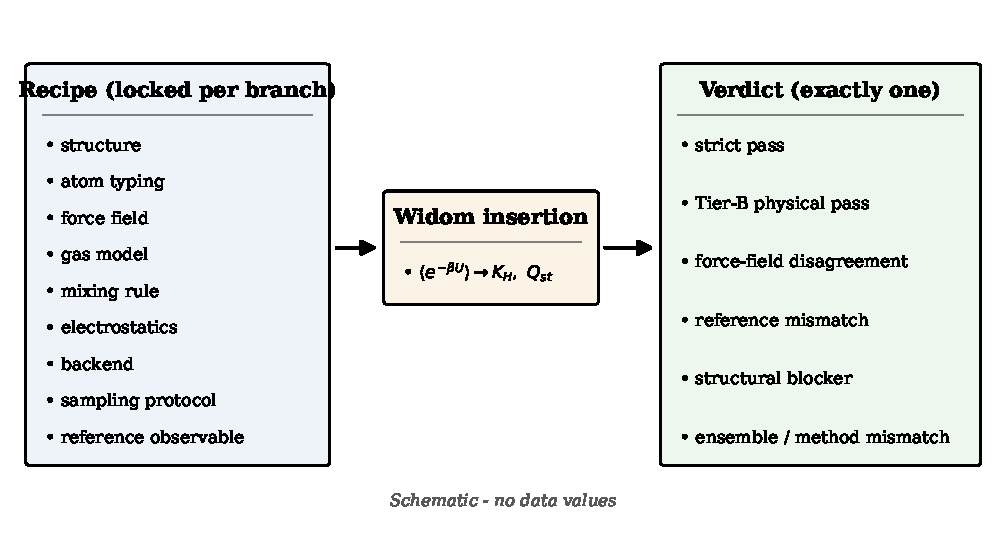
\includegraphics[width=0.92\textwidth]{figures/fig1_recipe_schematic.pdf}
\caption{A Widom adsorption number is the output of a complete recipe. The locked ingredients (left) feed Widom insertion (centre), whose zero-coverage \(K_H\) and \(Q_{st}\) are classified into exactly one of six verdicts (right). This figure is schematic and carries no numerical data.}
\label{fig:recipe}
\end{figure}

The first ingredient is the host structure. A zeolite topology name or a MOF name is not enough. The calculation needs the actual atomic coordinates, cell parameters, atom labels, and framework state. An all-silica CHA structure and a cationic chabazite are not the same material for carbon dioxide adsorption. A closed Na-Rho structure and an open Na-Rho adsorption state are not the same ensemble. A defective UiO-66 sample and an ideal UiO-66 crystal are not guaranteed to have the same low-pressure adsorption thermodynamics.

The second ingredient is the energy model. The force field defines how the guest sees the host. For a Lennard-Jones branch this means \(\epsilon\), \(\sigma\), charges, and the cross-pair rule. For Buckingham or exponential-attraction branches it means a different functional form and a different set of parameters. The gas model also matters: carbon dioxide can be represented by different charge distributions and Lennard-Jones sites, while methane can be a united-atom model or a more detailed model. These choices change \(U\), and therefore change both \(K_H\) and \(Q_{st}\).

The third ingredient is the long-range and truncation convention. Electrostatics may be absent, Ewald-summed, or represented differently by different engines. A Lennard-Jones cutoff may be used with or without an analytical tail correction. These are not cosmetic simulation settings. In the Si-CHA + CO\(_2\) branch, the analytical tail correction is part of the successful recipe because it shifts the Henry constant from the edge of the strict band into its interior.

The fourth ingredient is the backend. A backend is not merely a calculator button. It is the implementation that evaluates \(U\). RASPA3, RASPA2, the native widom-atlas evaluator, and the ASE-wrapper route can represent different subsets of force-field forms. A branch must therefore state which backend was used and why that backend is capable of representing the recipe.

The fifth ingredient is the reference observable. A number from the literature is not automatically the number that Widom insertion predicts. The reference may be a Henry slope, a Toth or Langmuir fit, a van't Hoff heat, a calorimetric heat, a finite-loading value, a breakthrough quantity, a site distance, or a kinetic parameter. widom-atlas treats these as different observables. It compares \(K_H\) and \(Q_{st}\) only when the reference can be defended as the same zero-coverage thermodynamic quantity.

This recipe view explains why branches, not materials, are the units of the atlas. MFI + CH\(_4\), MFI + Ar, and MFI + Kr share a framework family, but they are different recipes because the gas model, cross-pair parameters, reference values, and sometimes validation purpose differ. UiO-66 + CO\(_2\) also appears in more than one recipe because framework charges, explicit hydrogens, and literature reference choices change the calculation. The atlas must preserve those distinctions rather than average them away.

The recipe view also explains why a blocked branch is not a failed computation. If a cationic-zeolite reference has a clean Henry constant but the corresponding cation-containing CIF and cation force field are not locked, the scientific state is not ``FAIL''; it is ``not yet a defined calculation.'' If Na-Rho adsorption requires a gate-open framework state that rigid closed-state Widom does not sample, the scientific state is not ``bad parameter choice''; it is an ensemble mismatch. These labels prevent the atlas from manufacturing certainty where the recipe is incomplete.

For this reason, the case matrix is the scientific ledger of widom-atlas. It records the structure, atom typing, force-field form, gas model, mixing rule, electrostatics, backend, sampling protocol, reference observable, threshold, and verdict class for each branch. Once locked, the branch can be run, checked, and re-run. If the number changes without a recipe change, that is an implementation problem. If the number is stable but disagrees with the reference, the disagreement belongs to the recipe or to the reference, not to the Widom estimator in isolation.
